\begin{minipage}[c]{\textwidth}
\advance\leftskip-2.5cm
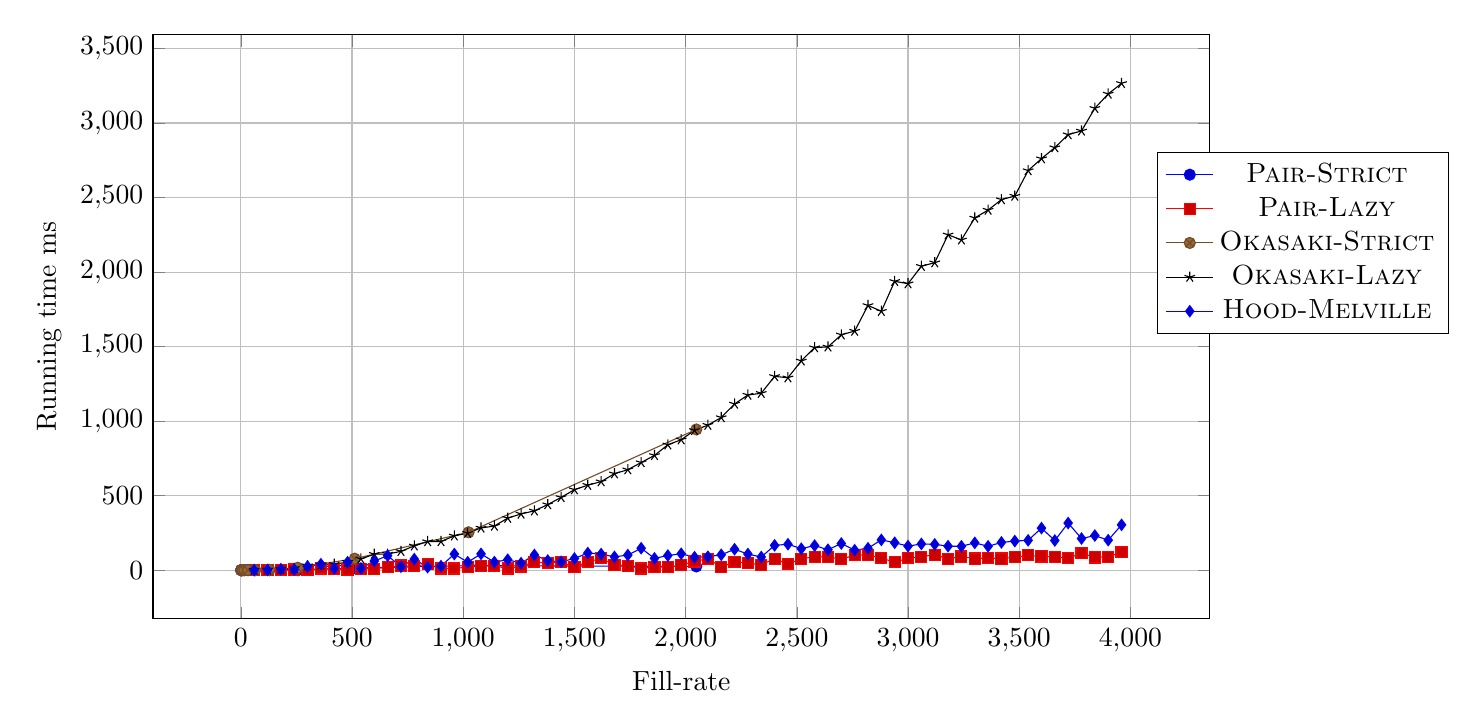
\begin{tikzpicture}
        \begin{axis}[
            xlabel = Fill-rate,
            ylabel = Running time ms,
            height=9cm,
            width=15cm,
            grid=major,
            legend style={
            at={(0.95,0.8)},
            anchor=north west}]            
            legend pos=center west
    	]
    		
  
                \addplot coordinates {
(1,0)
(2,0)
(4,0)
(8,0)
(16,0)
(32,1)
(64,0)
(128,0)
(256,0)
(512,14)
(1024,30)
(2048,25)

    	};
        
    	\addlegendentry{\textsc{Pair-Strict}}

        \addplot coordinates {
(60,1)
(120,1)
(180,0)
(240,4)
(300,2)
(360,11)
(420,8)
(480,4)
(540,10)
(600,9)
(660,20)
(720,31)
(780,26)
(840,40)
(900,11)
(960,11)
(1020,21)
(1080,29)
(1140,29)
(1200,11)
(1260,25)
(1320,53)
(1380,49)
(1440,52)
(1500,21)
(1560,55)
(1620,79)
(1680,35)
(1740,29)
(1800,11)
(1860,22)
(1920,20)
(1980,34)
(2040,58)
(2100,77)
(2160,21)
(2220,55)
(2280,46)
(2340,37)
(2400,76)
(2460,41)
(2520,77)
(2580,89)
(2640,90)
(2700,73)
(2760,101)
(2820,103)
(2880,81)
(2940,53)
(3000,80)
(3060,90)
(3120,104)
(3180,76)
(3240,91)
(3300,78)
(3360,82)
(3420,78)
(3480,86)
(3540,99)
(3600,92)
(3660,90)
(3720,80)
(3780,114)
(3840,85)
(3900,90)
(3960,119)

    	};
        
    	\addlegendentry{\textsc{Pair-Lazy}}

        \addplot coordinates {
(1,0)
(2,0)
(4,0)
(8,0)
(16,0)
(32,0)
(64,1)
(128,3)
(256,16)
(512,77)
(1024,254)
(2048,944)

    	};
        
    	\addlegendentry{\textsc{Okasaki-Strict}}

        \addplot coordinates {
(60,0)
(120,2)
(180,7)
(240,12)
(300,30)
(360,36)
(420,40)
(480,54)
(540,75)
(600,107)
(660,108)
(720,126)
(780,163)
(840,192)
(900,192)
(960,230)
(1020,248)
(1080,283)
(1140,296)
(1200,349)
(1260,377)
(1320,398)
(1380,440)
(1440,488)
(1500,540)
(1560,570)
(1620,594)
(1680,647)
(1740,674)
(1800,722)
(1860,770)
(1920,841)
(1980,875)
(2040,938)
(2100,973)
(2160,1024)
(2220,1115)
(2280,1175)
(2340,1187)
(2400,1300)
(2460,1291)
(2520,1404)
(2580,1493)
(2640,1498)
(2700,1579)
(2760,1604)
(2820,1776)
(2880,1737)
(2940,1938)
(3000,1922)
(3060,2039)
(3120,2063)
(3180,2250)
(3240,2216)
(3300,2363)
(3360,2416)
(3420,2486)
(3480,2510)
(3540,2681)
(3600,2761)
(3660,2835)
(3720,2922)
(3780,2947)
(3840,3099)
(3900,3195)
(3960,3266)

    	};
        
    	\addlegendentry{\textsc{Okasaki-Lazy}}

        \addplot coordinates {
(60,0)
(120,1)
(180,6)
(240,4)
(300,25)
(360,40)
(420,12)
(480,53)
(540,12)
(600,61)
(660,97)
(720,23)
(780,74)
(840,20)
(900,27)
(960,108)
(1020,53)
(1080,109)
(1140,54)
(1200,70)
(1260,47)
(1320,102)
(1380,64)
(1440,56)
(1500,78)
(1560,115)
(1620,108)
(1680,89)
(1740,101)
(1800,147)
(1860,79)
(1920,98)
(1980,110)
(2040,87)
(2100,90)
(2160,103)
(2220,140)
(2280,108)
(2340,88)
(2400,166)
(2460,174)
(2520,144)
(2580,165)
(2640,137)
(2700,179)
(2760,134)
(2820,147)
(2880,203)
(2940,184)
(3000,161)
(3060,176)
(3120,173)
(3180,161)
(3240,160)
(3300,183)
(3360,160)
(3420,186)
(3480,195)
(3540,200)
(3600,282)
(3660,199)
(3720,316)
(3780,212)
(3840,232)
(3900,201)
(3960,304)

    	};

    	\addlegendentry{\textsc{Hood-Melville}}

        \end{axis}

    \end{tikzpicture}
    \captionof{figure}{TITEL}
    \label{fig:sample_figure}
\end{minipage}